\begin{tabular}{M{7.5cm}M{10.5cm}}
	\textbf{TRUNG TÂM MANABIE}& \textbf{ĐỀ ÔN TẬP KIỂM TRA CUỐI HỌC KÌ 1}\\
	\textbf{MÃ ĐỀ: 005}& \textbf{Bài thi môn: VẬT LÝ 12}\\
	\textit{(Đề trường THPT Chuyên Phan Bội Châu - Nghệ An  năm học 2024 -2025)}& \textit{Thời gian làm bài: 50 phút, không kể thời gian phát đề}
	
	\noindent\rule{4cm}{0.8pt} \\
\end{tabular}
\setcounter{section}{0}
\section{Câu trắc nghiệm nhiều phương án lựa chọn}
\textit{Thí sinh trả lời từ câu 1 đến câu 18. Mỗi câu hỏi thí sinh chọn một phương án}
\setcounter{ex}{0}
\Opensolutionfile{ans}[ans/FINAL-SEM1-005-TN]
% ===================================================================
\begin{ex}
	Quá trình cục nước đá chuyến thành nước được gọi là quá trình
	\choice
	{đông đặc}
	{\True nóng chảy}
	{bay hơi}
	{ngưng kết}
	\loigiai{}
\end{ex}
% ===================================================================
\begin{ex}
	Biển báo nào dưới đây cảnh báo khu vực có nồng độ tia tử ngoại cao
	\choice
	{
\includegraphics[scale=0.5]{../figs/FINAL-SEM1-005-1}}
	{\True 
\includegraphics[scale=0.6]{../figs/FINAL-SEM1-005-2}}
	{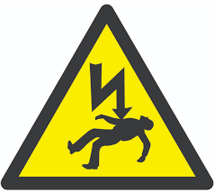
\includegraphics[scale=0.3]{../figs/FINAL-SEM1-005-3}}
	{
\includegraphics[scale=0.3]{../figs/FINAL-SEM1-005-4}}
	\loigiai{}
\end{ex}
\textit{Sử dụng các thông tin sau cho câu 3, câu 4 và câu 5:}
\immini{Hình vẽ bên là hình ảnh của quạt điều hoà (còn gọi là quạt nước) và các tấm Cooling Pad. Cấu tạo của quạt có 5 bộ phận chính gồm: bình nước, máy phun hơi nước, tấm Cooling Pad, tấm giữ bụi, động cơ gắn với cánh quạt. Tấm Cooling Pad chính là bộ phận quan trọng, được thiết kế dưới dạng hình khối chữ nhật với các rãnh nhằm tiếp xúc với nước, đồng thời giữ nước lại. Tấm màng này chiết xuất từ vỏ cây nên khả năng thẩm thấu tương đối nhanh.}
{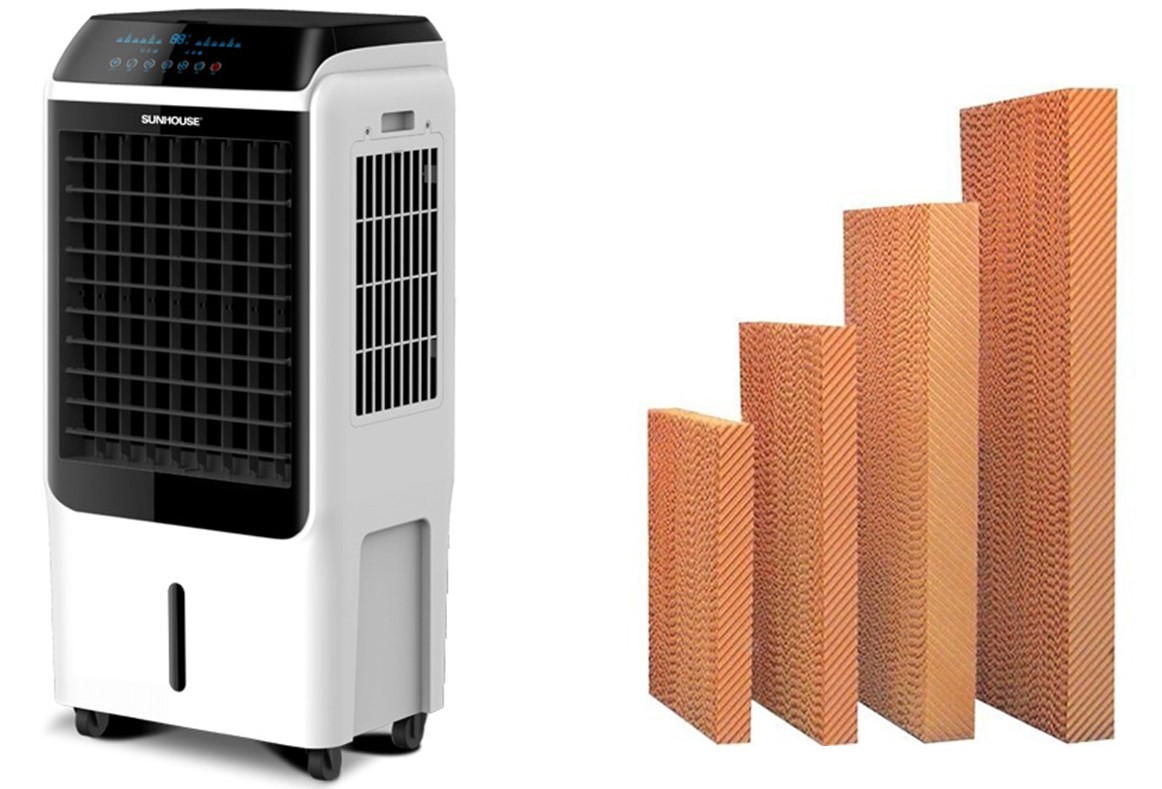
\includegraphics[scale=0.2]{../figs/FINAL-SEM1-005-5}}
% ===================================================================
\begin{ex}
Khi hệ thống làm mát hoạt động, các rãnh của tấm Cooling Pad tiếp xúc với nước, đồng thời nước được giữ lại và nhiệt độ của nước sẽ thay đổi thế nào?	
	\choice
	{tăng lên}
	{\True giảm xuống}
	{hạ xuống dưới \SI{0}{\celsius}}
	{không thay đổi}
	\loigiai{}
\end{ex}
% ===================================================================
\begin{ex}
	Khi động cơ của quạt hoạt động thì động cơ đã chuyển hóa phần lớn
	\choice
	{cơ năng thành điện năng}
	{điện năng thành nhiệt năng}
	{\True điện năng thành cơ năng}
	{nhiệt năng thành điện năng}
	\loigiai{}
\end{ex}
% ===================================================================
\begin{ex}
	Khi quạt hoạt động thì không khí sau khi đi qua quạt so với trước đó lượng hơi nước trong không khí
	\choice
	{\True tăng lên và nhiệt độ giảm xuống}
	{giảm xuống và nhiệt độ giảm xuống}
	{giảm xuống và nhiệt độ không đổi}
	{tăng lên và nhiệt độ không đổi}
	\loigiai{}
\end{ex}
% ===================================================================
\begin{ex}
	Sóng điện từ truyền trong chân không có bước sóng \SI{900}{\nano\meter} thuộc loại tia nào sau đây?
	\choice
	{Tia tử ngoại}
	{Tia X}
	{\True Tia hồng ngoại}
	{Tia gamma ($\gamma$)}
	\loigiai{}
\end{ex}
% ===================================================================
\begin{ex}
Một bạn học sinh dùng bơm có van một chiều để bơm không khí vào một quả bóng. Ban đầu quả bóng chứa không khí ở áp suất khí quyển $p_0$. Bóng có thể tích không đổi $V$. Coi nhiệt độ không khí trong và ngoài bóng như nhau và không đổi. Mỗi lần bơm đưa được một thể tích bằng $0,2V$ không khí vào bóng. Sau lần bơm đầu tiên, áp suất không khí trong bóng là	
	\choice
	{$p=\dfrac{p_0}{1,2}$}
	{$p=1,44p_0$}
	{\True $p=1,2p_0$}
	{$p=\dfrac{p_0}{1,44}$}
	\loigiai{
	$pV=const\Rightarrow p_0\left(V+0,2V\right)=pV\Rightarrow p=1,2p_0$.
	}
\end{ex}
% ===================================================================
\begin{ex}
	Một khối khí lí tưởng được giữ ở áp suất không đổi. Nếu làm cho nhiệt độ tuyệt đối của khối khí này tăng lên hai lần so với giá trị ban đầu thì thể tích khí bằng
	\choice
	{một phần tư giá trị ban đầu}
	{một nửa giá trị ban đầu}
	{bốn lần so với giá trị ban đầu}
	{\True hai lần so với giá trị ban đầu}
	\loigiai{}
\end{ex}
% ===================================================================
\begin{ex}
Một khối khí lí tưởng có $n$ mol khí, có nhiệt độ tuyệt đối $T$, có thể tích $V$ thì áp suất $p$ tác dụng lên thành bình là	
	\choice
	{$p=\dfrac{nV}{RT}$}
	{$p=\dfrac{RT}{nV}$}
	{$p=\dfrac{V}{nRT}$}
	{\True $p=\dfrac{nRT}{V}$}
	\loigiai{}
\end{ex}
\immini{\textit{Sử dụng các thông tin sau cho câu 10 , câu 11 và câu 12 . Hình vẽ bên là hình ảnh sóng hình sin truyền trên một sộ dây đàn hồi rất dài tù đầu 0 (được căng ngang) tại hai thời điểm $t_1$ và $t_2$.}}
{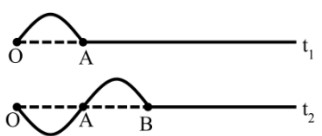
\includegraphics[scale=0.9]{../figs/FINAL-SEM1-005-6}}
% ===================================================================
\begin{ex}
	Chu kì sóng trên dây là
	\choice
	{$T=t_2-t_1$}
	{$T=0,5\left(t_2-t_1\right)$}
	{$T=4\left(t_2-t_1\right)$}
	{\True $T=2\left(t_2-t_1\right)$}
	\loigiai{$t_2-t_1=\dfrac{T}{2}\Rightarrow T=2\left(t_2-t_1\right)$.}
\end{ex}
% ===================================================================
\begin{ex}
	Bước sóng trên dây có giá trị bằng
	\choice
	{hai lần độ dài đoạn OB}
	{\True độ dài đoạn OB}
	{độ dài đoạn OA}
	{một nửa độ dài đoạn OA}
	\loigiai{}
\end{ex}
% ===================================================================
\begin{ex}
	Tại thời điểm $t_2$, các phần tử dây tại O, A, B chuyển động như thế nào?
	\choice
	{O, A, B đều đang đi lên}
	{\True O và B đang đi lên, A đang đi xuống}
	{O và A đang đi lên, B đang đi xuống}
	{O, A, B đều đang đi xuống}
	\loigiai{}
\end{ex}
\textit{Sử dụng các thông tin ở bảng bên cho các câu 13 và câu 14.}
\begin{center}
	\begin{tabular}{|L{3cm}|M{5cm}|L{3cm}|M{5cm}|}
		\hline
		\thead{Chất} & \thead{Nhiệt dung riêng\\ $\left(\si{\joule/\kilogram\cdot\kelvin}\right)$} & \thead{Chất} & \thead{Nhiệt dung riêng\\ $\left(\si{\joule/\kilogram\cdot\kelvin}\right)$}\\
		\hline
		Nhôm & 880 & Đất & 800\\
		\hline
		Sắt & 460 & Nước đá & 2100\\
		\hline
		Đồng & 380 & Nước & 4180\\
		\hline
		Chì & 130 & Rượu & 2500\\
		\hline
	\end{tabular}
\end{center}
% ===================================================================
\begin{ex}
Nhiệt lượng cần cung cấp cho \SI{2}{\kilogram} rượu nóng thêm \SI{1}{\celsius} là	
	\choice
	{\SI{1250}{\joule}}
	{\SI{4180}{\joule}}
	{\SI{2500}{\joule}}
	{\True \SI{5000}{\joule}}
	\loigiai{
	$Q=mc\Delta t=2\cdot2500\cdot1=\SI{5000}{\joule}$.
	}
\end{ex}
% ===================================================================
\begin{ex}
Các miếng Nhôm, Đồng, Sắt và Chì có cùng khối lượng. Nếu lần lượt cung cấp cho các miếng kim loại trên một nhiệt lượng như nhau thì miếng kim loại nào tăng nhiệt độ nhiều nhất?	
	\choice
	{Đồng}
	{\True Chì}
	{Sắt}
	{Nhôm}
	\loigiai{
	$Q=mc\Delta t\Rightarrow\Delta t=\dfrac{Q}{mc}\Rightarrow c$ càng nhỏ thì $\Delta t$ càng lớn.
	}
\end{ex}
% ===================================================================
\begin{ex}
	\immini{ Sự chuyển động liên tục của ong vò vẽ làm nó tích điện và tự tạo ra xung quanh mình một điện trường. Khi đậu vào bông hoa nó truyền cho bông hoa một điện tích. Ong vò vẽ tìm được mật hoa và phân biệt được hoa tươi với hoa đã hết mật là nhờ vào tính chất nào sau đây?}
	{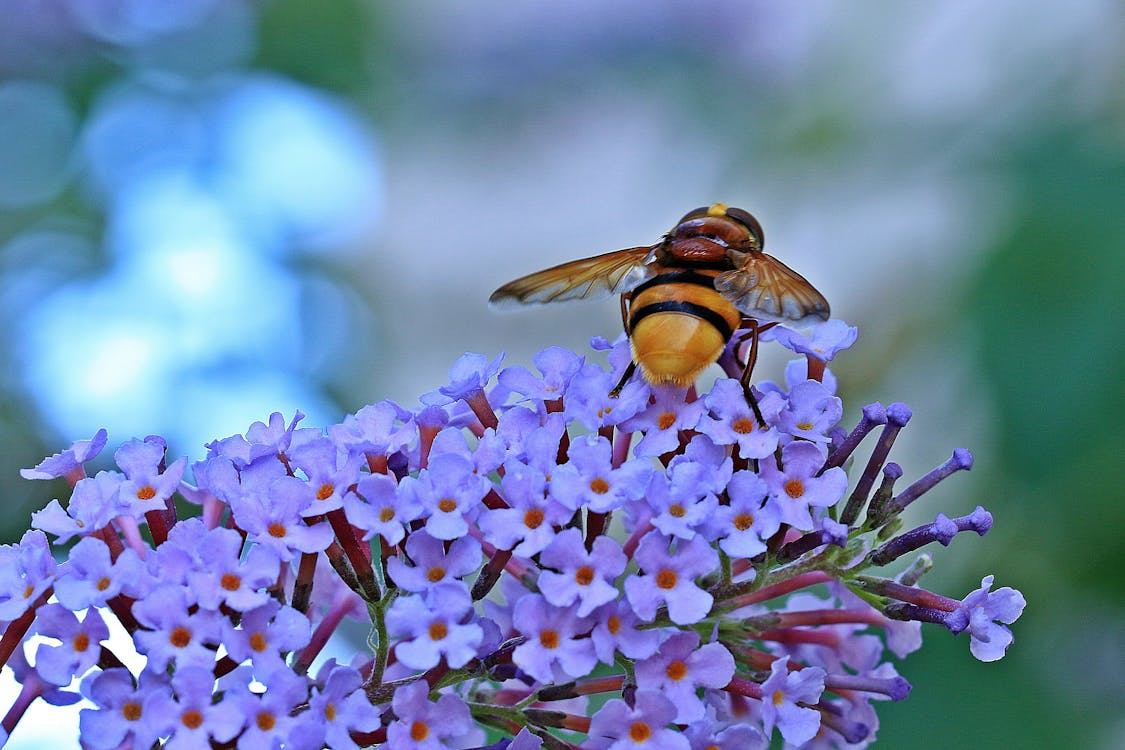
\includegraphics[scale=0.08]{../figs/FINAL-SEM1-005-7}}
	\choice
	{Lực hút giữa điện tích trên bông hoa và điện tích trên cái râu của ong vò vẽ}
	{\True Lực đẩy giữa điện tích trên bông hoa và điện tích trên cái râu của ong vò vẽ}
	{Ong vò vẽ phát ra hạ âm và hạ âm bị phản xạ khi gặp bông hoa}
	{Ong vò vẽ phát ra âm thanh và âm bị phản xạ khi gặp bông hoa}
	\loigiai{}
\end{ex}
% ===================================================================
\begin{ex}
	Phương pháp nào sau đây không làm tăng nội năng của vật?
	\choice
	{Nước trong nồi được đun nóng}
	{Cọ xát miếng kim loại vào mặt bàn}
	{Viên bi được thả vào nước nóng}
	{\True Viên bi rơi trong chân không}
	\loigiai{}
\end{ex}
% ===================================================================
\begin{ex}
	 Một dây dẫn hình trụ bằng đồng và một dây dẫn hình trụ bằng nhôm có cùng kích thước. Nếu đặt vào hai đầu mỗi dây cũng một hiệu điện thế thì tỷ số giữa công suất toả nhiệt trên dây đồng và công suất toả nhiệt trên đây nhôm xấp xỉ bằng
	\choice
	{0,61}
	{2,65}
	{\True 1,63}
	{0,38}
	\loigiai{
	$R=\dfrac{\rho\ell}{S}\Rightarrow \dfrac{R_{\ce{Al}}}{R_{\ce{Cu}}}=\dfrac{\rho_{\ce{Al}}}{\rho_{\ce{Cu}}}=\dfrac{2,75\cdot10^{-8}}{1,69\cdot10^{-8}}\approx1,63$.\\
	$\calP=\dfrac{U^2}{R}\Rightarrow \dfrac{\calP_{\ce{Cu}}}{\calP_{\ce{Al}}}=\dfrac{R_{\ce{Al}}}{R_{\ce{Cu}}}\approx1,63$.
	}
\end{ex}
% ===================================================================
\begin{ex}
	Bốn vật dẫn hình trụu có cùng kích thước được chế tạo bằng bạc $\left(\ce{Ag}\right)$, đồng $\left(\ce{Cu}\right)$, nhôm $\left(\ce{Al}\right)$, sắt $\left(\ce{Fe}\right)$. Lần lượt nối vào hai đầu mỗi vật đẫn cùng một nguồn điện có suất điện động không đổi thì dòng điện chạy trong dây dẫn nào có cường độ lớn nhất?
	\choice
	{Dây dẫn bằng \ce{Cu}}
	{Dây dẫn bằng \ce{Al}}
	{Dây dẫn bằng \ce{Fe}}
	{Dây dẫn bằng \ce{Ag}}
	\loigiai{
	$I=\dfrac{U}{R}=\dfrac{U}{\dfrac{\rho\ell}{S}}\Rightarrow I$ lớn nhất khi $\rho$ nhỏ nhất.
	}
\end{ex}
\Closesolutionfile{ans}
\section{Câu trắc nghiệm đúng/sai} 
\textit{Thí sinh trả lời từ câu 1 đến câu 4. Trong mỗi ý \textbf{a)}, \textbf{b)}, \textbf{c)}, \textbf{d)} ở mỗi câu, thí sinh chọn đúng hoặc sai}
\setcounter{ex}{0}
\Opensolutionfile{ans}[ans/FINAL-SEM1-005-TF]
% ===================================================================
\begin{ex}
	\immini{Cây đàn Nguyệt là một nhạc cụ dân tộc, dây đàn chỉ là một dây cước, hộp đàn có dạng hình mặt nguyệt. Khi gảy đàn, ứng với các nốt nhạc khác nhau thì người ta bấm tay vào các phím đàn khác nhau (như hình bên).}
	{\vspace{-0.5cm}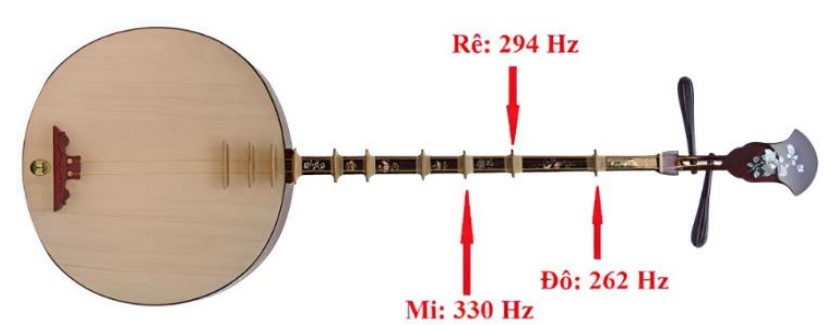
\includegraphics[scale=0.5]{../figs/FINAL-SEM1-005-8}}
	\choiceTF[t]
	{\True Hộp đàn có chức năng cộng hưởng âm}
	{\True Khi gảy vào dây đàn thì dao động được truyền đi dưới dạng sóng ngang về hai đầu dây, chúng bị phản xạ và truyền theo chiều ngược lại tạo ra sóng dừng trên đây đàn}
	{Tốc độ truyền dao động trên dây đàn $v=\sqrt{\dfrac{F}{m_0}}$ trong đó $F$ là lực căng dây, còn $m_0$ là khối lượng trên một đơn vị chiều dài của dây. Dây đàn dài \SI{750}{\milli\meter}, nặng \SI{25}{\gram}, lực căng \SI{4320}{\newton}. Khi không bấm nốt thì âm mà dây đàn này phát ra có tần số \SI{162}{\hertz}}
	{\True Sau khi căn chỉnh lại lực căng dây, nếu khoảng cách từ phím đàn ứng với nốt Đô (có tần số \SI{262}{\hertz}) đến phím đàn ứng với nốt Rê (có tần số \SI{294}{\hertz}) là \SI{80.0}{\milli\meter} thì khoảng cách từ phím đàn ứng với nốt Rê (có tần số \SI{294}{\hertz}) đến phím đàn ứng với nốt Mi (có tần số \SI{330}{\hertz}) là \SI{71.5}{\milli\meter}}
	\loigiai{\begin{itemchoice}
			\itemch Đúng.
			\itemch Đúng.
			\itemch Sai. $m_0=\dfrac{25\cdot10^{-3}}{750\cdot10^{-3}}=\xsi{\dfrac{1}{30}}{\kilogram/\meter}$;\\
			$v=\sqrt{\dfrac{F}{m_0}}=\sqrt{\dfrac{4320}{1/30}}=\SI{360}{\meter/\second}$;\\
			$f_c=\dfrac{v}{2\ell}=\dfrac{360}{2\cdot750\cdot10^{-3}}=\SI{240}{\hertz}$.
			\itemch Đúng.\\
			$\begin{cases}
				\ell_{\text{Đô}}-\ell_{\text{Rê}}=\dfrac{v}{2f_{\text{Đô}}}-\dfrac{v}{2f_{\text{Rê}}}\\
				\ell_{\text{Rê}}-\ell_{\text{Mi}}=\dfrac{v}{2f_{\text{Rê}}}-\dfrac{v}{2f_{\text{Mi}}}
			\end{cases}\Rightarrow \dfrac{\ell_{\text{Đô}}-\ell_{\text{Rê}}}{\ell_{\text{Rê}}-\ell_{\text{Mi}}}=\dfrac{\dfrac{1}{f_{\text{Đô}}}-\dfrac{1}{f_{\text{Rê}}}}{\dfrac{1}{f_{\text{Rê}}}-\dfrac{1}{f_{\text{Mi}}}}\Rightarrow \dfrac{80}{\ell_{\text{Rê}}-\ell_{\text{Mi}}}=\dfrac{\dfrac{1}{262}-\dfrac{1}{294}}{\dfrac{1}{294}-\dfrac{1}{330}}$\\
			$\Rightarrow \ell_{\text{Rê}}-\ell_{\text{Mi}}\approx\SI{71.5}{\milli\meter}.$
	\end{itemchoice}}
\end{ex}
% ===================================================================
\begin{ex}
	Một nhóm học sinh lớp 12A một trường THPT thực hiện thí nghiệm thực hành đo nhiệt dung riêng của nước.\\
	Họ đã lựa chọn bộ dụng cụ thì nghiệm gồm: biến thể nguồn (1), bộ đo công suất nguồn điện (oát kế có độ chính xác là \SI{0.1}{\watt}) có tích hợp chức năng đo thời gian (2), nhiệt kế điện tử (3) có độ chính xác là \SI{0.1}{\celsius}, nhiệt lượng kế bằng nhựa có vỏ xốp kèm dây điện trở (4), cân điện tử (5) có độ chính xác \SI{0.01}{\gram} như hình vẽ.\\
	Họ đã lựa chọn phương án thí nghiệm: đo nhiệt lượng $Q$ cung cấp cho khối lượng nước $m$ để làm tăng nhiệt độ của nó lên $\Delta t$ và tính nhiệt dung riêng theo công thức: $c=\dfrac{Q}{m \cdot \Delta t}$.\\
	Thí nghiệm được tiến hành với khối lượng nước là \SI{145.62}{\gram} và nhiệt độ ban đầu của nước là \SI{9.6}{\celsius}. Nhóm học sinh này đã xác định được tổng nhiệt dung (nhiệt lượng cần cung cấp cho 1 vật để nhiệt độ của nó tăng thêm một độ) của bộ dụng cụ kèm theo (gồm bình nhiệt lượng kế, dây điện trở và thanh dẫn, nhiệt kế và que khuấy) là $c_0=\SI{44.3}{\joule/\kelvin}$. Bảng số liệu đo được như ở hình bên dưới
	\begin{center}
		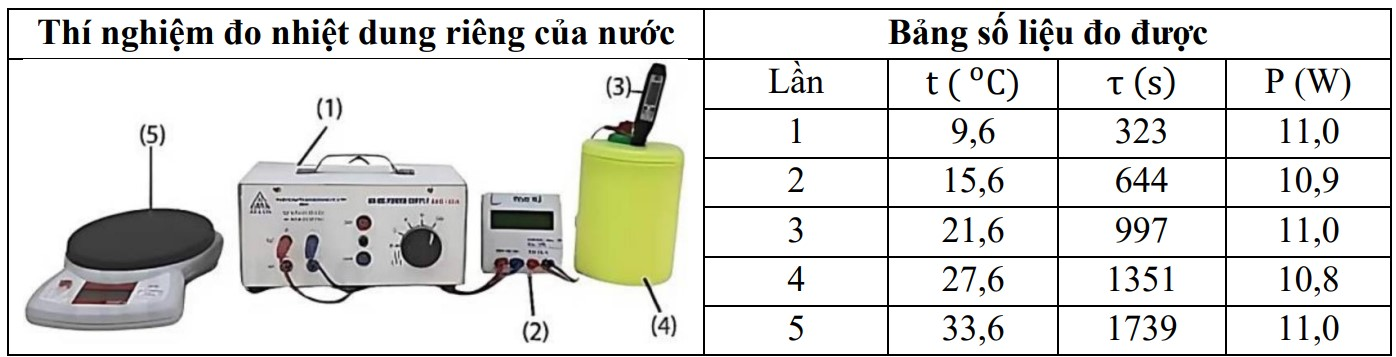
\includegraphics[scale=0.5]{../figs/FINAL-SEM1-005-10}
	\end{center}
	\choiceTF[t]
	{\True Công suất toả nhiệt trung bình của dây điện trở là \SI{10.9}{\watt}}
	{Sai số tỷ đối của phép đo độ chênh lệch nhiệt độ giữa hai lần đo liên tiếp do dụng cụ đo (nhiệt kế điện tử) gây ra là \SI{2.67}{\percent}}
	{\True Gọi độ tăng nhiệt độ ở hai lần đo liên tiếp là $\Delta t$ (độ) và khoảng thời gian ở hai lần đo liên tiếp là $\xsi{\Delta \tau}{\left(\second\right)}{}$. Giá trị trung bình của tỷ số giữa $\Delta t$ và $\Delta \tau$ trong thí nghiệm là \SI{0.017}{\text{độ}/\second}}
	{Từ kết quả thí nghiệm, giá trị trung bình của nhiệt dung riêng của nước đo được là $c=\SI{4100}{\joule/\kilogram\cdot\kelvin}$}
	\loigiai{\begin{itemchoice}
			\itemch Đúng. $\overline{\calP}=\dfrac{\calP_1+\calP_2+\dots+\calP_5}{5}\approx\SI{10.9}{\watt}$.
			\itemch Sai. Đặt $T$ là độ chênh lệch nhiệt độ giữa hai lần đo liên tiếp
			\begin{center}
				\begin{tabular}{|M{5cm}|M{5cm}|M{5cm}|}
					\hline
					$\xsi{T}{\left(\si{\celsius}\right)}$ & 	$\xsi{\Delta \tau}{\left(\si{\celsius}\right)}$ & 	$\xsi{\dfrac{T}{\Delta \tau}}{\left(\si{\celsius/\second}\right)}$\\
					\hline
					$15,6-9,6=6$ & $644-323=321$ & $6/321$\\
					\hline
					$21,6-15,6=6$ & $997-644=353$ & $6/353$\\
					\hline
					$27,6-21,6=6$ & $1351-997=354$ & $6/354$\\
					\hline
					$33,6-27,6=6$ & $1739-1351=388$ & $6/388$\\
					\hline
				\end{tabular}
			\end{center}
			$\begin{cases}
				t_1=9,6\pm0,1\\
				t_2=15,6\pm0,1\\
				t_3=21,6\pm0,1\\
				t_4=27,6\pm0,1\\
				t_5=33,6\pm0,1
			\end{cases}\Rightarrow \delta T=\dfrac{\Delta T}{\overline{T}}\cdot\SI{100}{\percent}=\dfrac{\left(0,1+0,1\right)}{6}\cdot\SI{100}{\percent}\approx\SI{3.33}{\percent}$.
			\itemch Đúng. $\dfrac{\overline{T}}{\Delta \tau}=\dfrac{\dfrac{6}{321}+\dfrac{6}{353}+\dfrac{6}{354}+\dfrac{6}{388}}{4}\approx\SI{0.017}{\text{độ}/\second}$.
			\itemch Sai. $\calP\Delta\tau=\left(mc+c_0\right)\Delta t\Rightarrow 10,94\cdot\left(1739-323\right)=\left(145,62\cdot10^{-3}\cdot c+44,3\right)\cdot\left(33,6-9,6\right)\Rightarrow c\approx\SI{4128}{\joule/\kilogram\cdot\kelvin}$.
	\end{itemchoice}}
\end{ex}
% ===================================================================
\begin{ex}
	\immini{Máy khử rung tim xách tay là thiết bị được các đội y tế thường dùng để cấp cứu bệnh nhân bị rối loạn nhịp tim và tạo nhịp tim ổn định cho bệnh nhân. Để cấp cứu cho bệnh nhân, nhân viên y tế đặt hai điện cực của máy khử rung tim lên ngực bệnh nhân và truyền năng lượng dự trữ trong tụ điện cho bệnh nhân. Giả sử tụ điện trong máy có điện dung \SI{60}{\micro\farad} và hiệu điện thế giữa hai bản tụ điện là \SI{4000}{\volt}.}
	{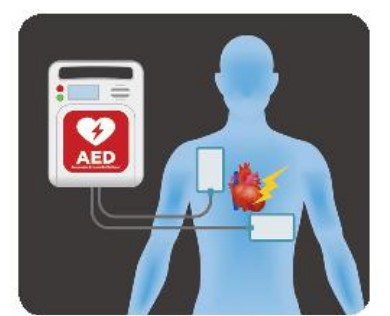
\includegraphics[scale=0.5]{../figs/FINAL-SEM1-005-11}}
	\choiceTF[t]
	{\True Khi máy hoạt động năng lượng truyền cho bệnh nhân là năng lượng của điện trường dự trữ trong tụ điện}
	{Với các thông số ở trên, điện tích của tụ điện trong máy khử rung tim là \SI{24E4}{\coulomb}}
	{Tụ điện dự trữ một năng lượng \SI{240}{\kilo\watt\hour}}
	{\True Giả sử trung bình máy truyền một xung đầu tiên trong thời gian \SI{2}{\milli\second} và truyền cho bệnh nhân một năng lượng khoảng \SI{200}{\joule}. Cường độ dòng điện trung bình chạy qua tim trong xung điện này là \SI{28.35}{\ampere}}
	\loigiai{\begin{itemchoice}
			\itemch Đúng. 
			\itemch Sai. $Q=CU=60\cdot10^{-6}\cdot4000=\SI{0.24}{\coulomb}$. 
			\itemch Sai. $W=\dfrac{1}{2}CU^2=\dfrac{1}{2}\cdot60\cdot10^{-6}\cdot4000^2=\SI{480}{\joule}$.
			\itemch Đúng. $W'=\dfrac{1}{2}\cdot\dfrac{q'^2}{C}\Rightarrow 480-200=\dfrac{1}{2}\cdot\dfrac{q'^2}{60\cdot10^{-6}}\Rightarrow q'=\xsi{0,04\sqrt{21}}{\coulomb}$.\\
			$i=\left|\dfrac{\Delta q}{\Delta t}\right|=\dfrac{0,24-0,04\sqrt{21}}{2\cdot10^{-3}}\approx\SI{28.35}{\ampere}$.
	\end{itemchoice}}
\end{ex}
% ===================================================================
\begin{ex}
	\immini{Khi lặn xuống biển để sửa chữa tàu biển, người nhái phải mang theo một bình không khí có thể tích không đổi tới áp suất \SI{150}{atm} để thở. Khi lặn xuống nước quan sát thân tàu và sau 8 phút thì tìm được chỗ hỏng (ở độ sâu \SI{5}{\meter} so với mặt biển), lúc ấy áp suất khí nén trong bình đã giảm bớt \SI{20}{\percent}. Người ấy tiến hành sửa chữa và từ lúc ấy tiêu thụ không khí gấp 1,5 lần so với lúc quan sát. Coi nhiệt độ không khí trong bình không đổi.}
	{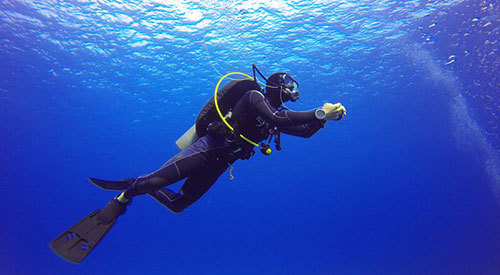
\includegraphics[scale=0.25]{../figs/FINAL-SEM1-005-12}}
	\choiceTF[t]
	{\True Người nhái lặn xuống càng sâu thì áp lực mà nước đè lên càng lớn}
	{\True Cho áp suất khí quyển là \SI{9.5}{\meter} nước biển. Tại vị trí thân tàu bị hỏng, áp suất nước biển là \SI{14.5}{\meter} nước biển}
	{Khi thở, người nhái thải ra các bọt khí có dạng hình cầu. Giả sử khi đang sửa thân tàu một bọt khí thở ra có bán kính $r_0$ (coi nhiệt độ của bọt khí không đổi), lúc nổi lên sát mặt thoáng thì bọt khí có bán kính $1,5r_0$}
	{Vì lí do an toàn cho phép là áp suất khí trong bình không thấp hơn \SI{30}{atm}. Người nhái có thể sửa chữa thân tàu trong thời gian tối đa là 20 phút}
	\loigiai{\begin{itemchoice}
			\itemch Đúng. 
			\itemch Đúng. Tại vị trí thân tàu bị hỏng, áp suất nước biển là $9,5+5=\SI{14.5}{\meter}$ nước biển.
			\itemch Sai. $p_1V_1=p_2V_2\Rightarrow 14,5\cdot\dfrac{4}{3}\pi r^3_0=9,5\cdot\dfrac{4}{3}\pi r^3\Rightarrow r\approx1,15r_0$.
			\itemch Sai. 8 phút quan sát thì áp suất đã mất đi $150\cdot0,2=\SI{30}{atm}$ và còn lại $150-30=\SI{120}{atm}\Rightarrow$ 8 phút sửa chữa thì áp suất mất đi $30\cdot1,5=\SI{45}{atm}$.\\
			Người nhái có thể sửa chữa thân tàu trong thời gian tối đa là $\dfrac{\left(120-30\right)}{45}\cdot8=\SI{16}{\minute}$.
	\end{itemchoice}}
\end{ex}
\Closesolutionfile{ans}
\section{Câu trắc nghiệm trả lời ngắn} \textit{Thí sinh trả lời từ câu 1 đến câu 6}
\setcounter{ex}{0}
\Opensolutionfile{ans}[ans/FINAL-SEM1-005-TL]
% ===============================================================
\begin{ex}
	Một nhóm học sinh tiến hành thí nghiệm giao thoa ánh sáng bằng hai khe. Nguồn sáng phát ra hai ánh sáng đơn sắc là ánh sáng vàng có bước sóng $\lambda_1$ và ánh sáng có bước sóng $\lambda_2$. Các bạn học sinh tiến hành đo khoảng vân của ánh sáng màu vàng, từ đó tính được bước sóng $\lambda_1=\SI{0.60}{\micro\meter}$. Khi quan sát trên màn, các bạn nhận thấy tại vị trí vân tối thứ 2 của ánh sáng vàng (kể từ vân trung tâm) là một vân sáng của $\lambda_2$. Giá trị $\lambda_2$ là bao nhiêu \si{\micro\meter}? (lấy đến hai chữ số sau dấu phẩy).
	\shortans[oly]{0,45}
	\loigiai{
		$k_1\lambda_1=k_2\lambda_2\xrightarrow[]{0,38\le \lambda_2\le 0,76}1,18\le k_2\le 2,37\Rightarrow k_2=2\Rightarrow\lambda_2=\SI{0.45}{\micro\meter}$.
	}
\end{ex}
% ===============================================================
\begin{ex}
	Xe ô tô điện VF6 của hãng xe Vinfat sử dụng loại pin hoá học LFP dung lượng \SI{59.6}{\kilo\watt\hour}. 
\immini{Khi xe chạy với tốc độ \SI{60}{\kilo\watt\hour} trên một cung đường bằng phẳng với công suất cơ học trung bình \SI{5.1}{\kilo\watt} chiếm \SI{60}{\percent} công suất xả của pin (ngoài điện năng cung cấp cho động cơ, pin còn cung cấp năng lượng cho hệ thống sưởi không khí khi xe chạy vào mùa đông, năng lượng cung cấp cho hệ thống vận hành túi khí,\dots) và xe chỉ vận hành khi dung lượng của pin còn lớn hơn \SI{20}{\percent} dung lượng ban đầu.}
{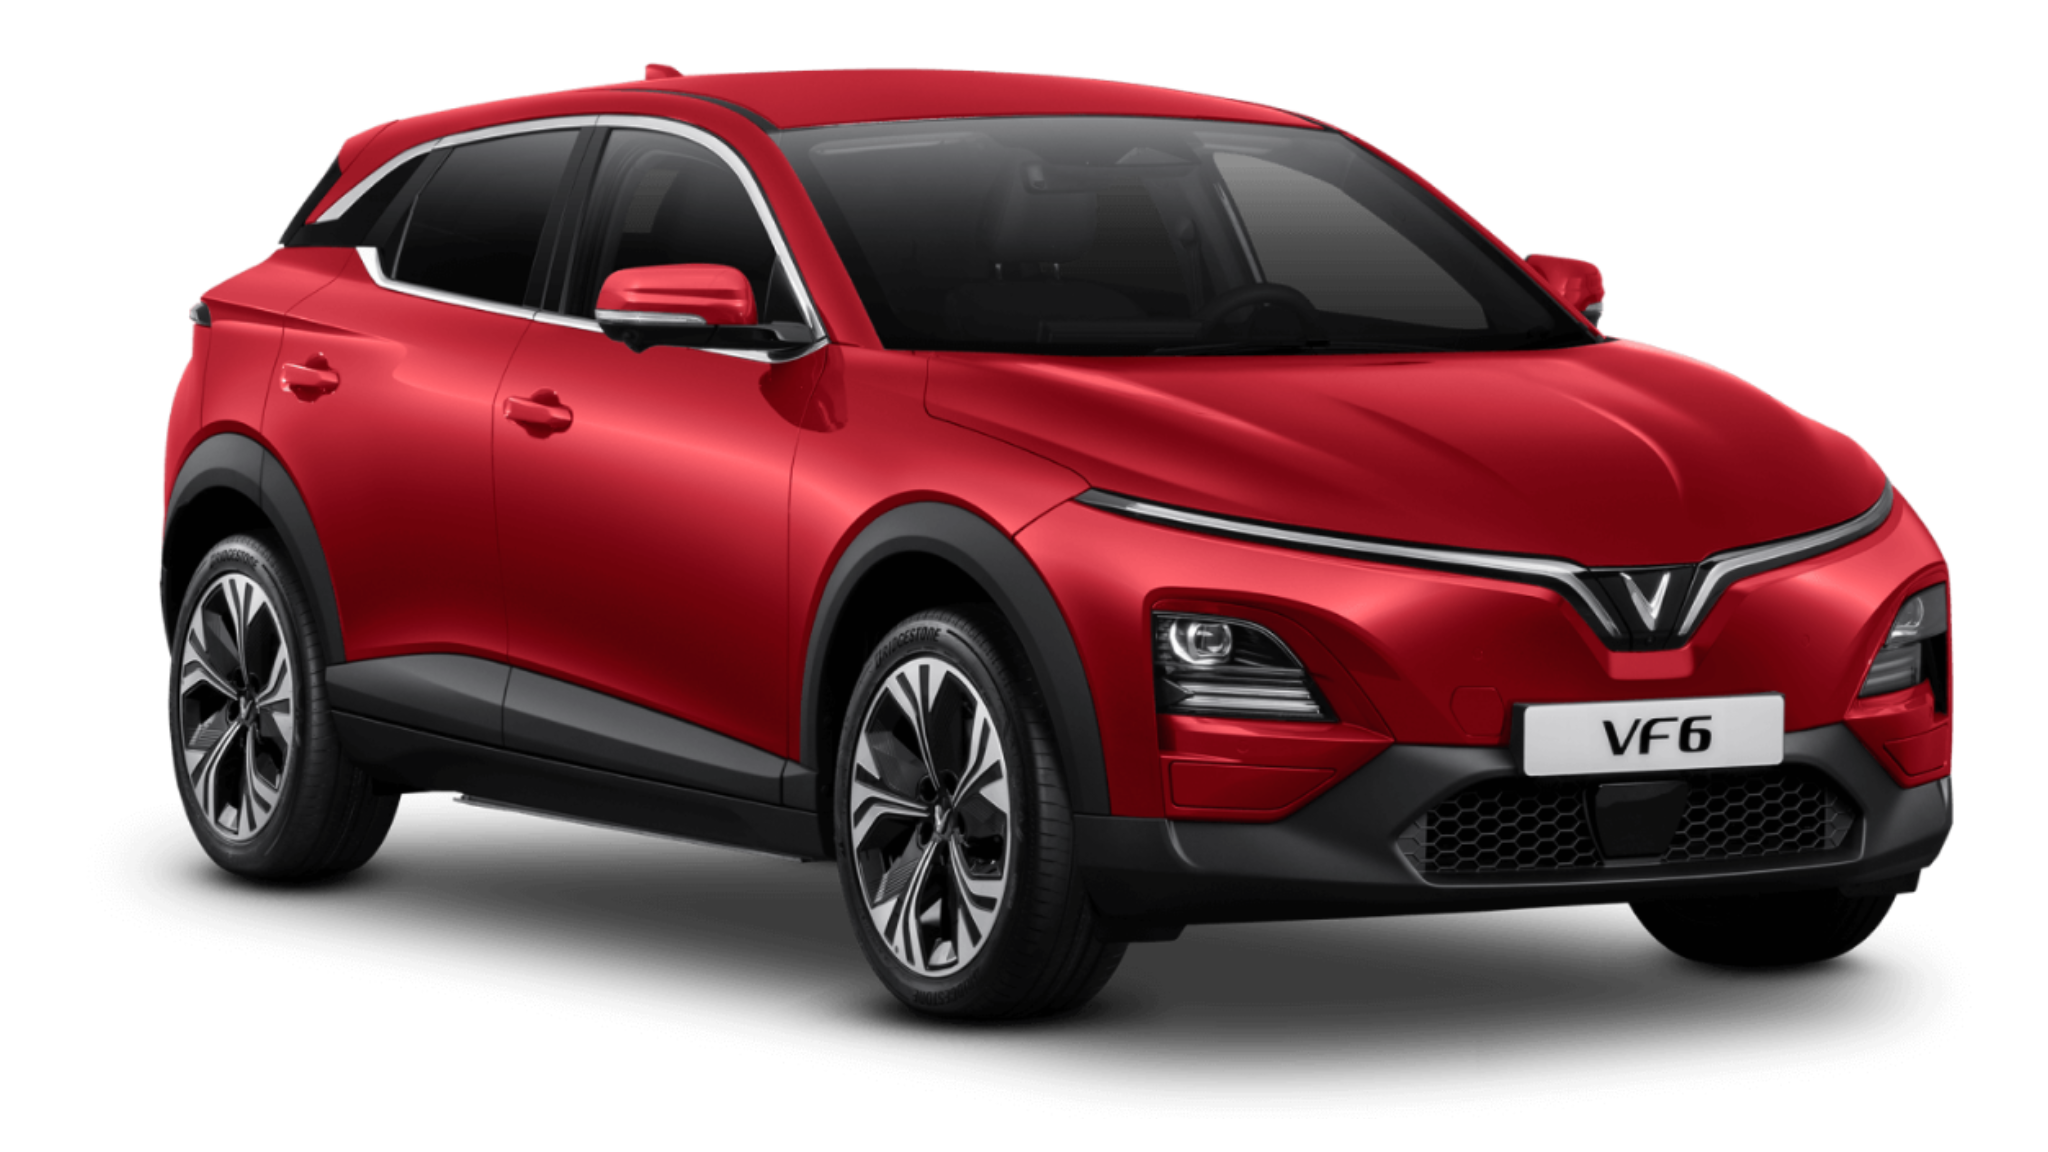
\includegraphics[scale=0.06]{../figs/FINAL-SEM1-005-13}}
Sau mỗi lần sạc pin thì xe vận hành được bao nhiêu \si{\kilo\meter}? (lấy đến chữ số hàng đơn vị).
	\shortans[oly]{337}
	\loigiai{
	Dung lượng pin tiêu thụ $A=\left(1-0,2\right)\cdot59,6=\SI{47.68}{\kilo\watt\hour}$.\\\
	Công cơ học là $A_C=HA=0,6\cdot 47,68=\SI{28.608}{\kilo\watt\hour}$.\\
	Thời gian $t=\dfrac{A_C}{\calP_C}=\dfrac{18,608}{5,1}\approx\SI{5.61}{\hour}$.\\
	Quãng đường $s=vt=60\cdot5,61=\SI{336.6}{\kilo\meter}$.	
	}
\end{ex}
% ===============================================================
\begin{ex}
	\immini{Hương vị của bia Hà nội đã trở thành một thương hiệu mà nhiều người yêu thích. Mở nắp một chai bia rồi rót \SI{200}{\gram} bia vào cốc. Cho vào cốc \SI{40}{\gram} nước đá ở nhiệt độ \SI{-2.8}{\celsius} thì ta sẽ được một cốc bia mát. Biết nhiệt dung riêng của bia là \SI{3830}{\joule/\kilogram\cdot\kelvin}, nhiệt dung riêng của nước đá là \SI{1800}{\joule/\kilogram\cdot\kelvin}; nhiệt nóng chảy riêng của nước đá là \SI{3.4E5}{\joule/\kilogram}, nhiệt dung riêng của nước là \SI{4200}{\joule/\kilogram\cdot\kelvin}. }
	{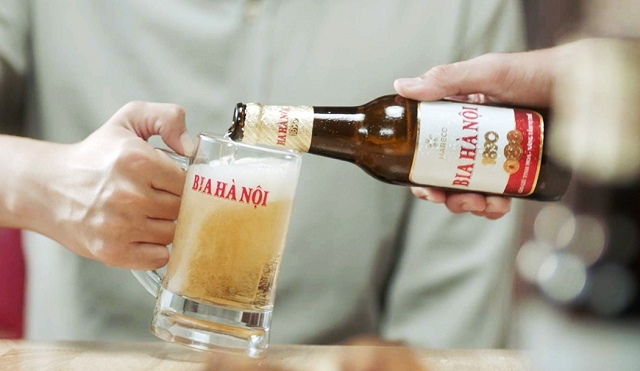
\includegraphics[scale=0.2]{../figs/FINAL-SEM1-005-14}}
	Ban đầu bia có nhiệt độ là \SI{32}{\celsius}. Bỏ qua sự trao đổi nhiệt với môi trường và sự trao đổi nhiệt với thành cốc. Sau khi nước đá tan hết, nhiệt độ của cốc bia là bao nhiêu \si{\celsius}? (lấy đến một chữ số sau dấu phẩy).
	\shortans[oly]{11,5}
	\loigiai{
		$m_d\left(c_d\Delta t_d+\lambda+c_n\Delta t_c\right)=m_bc_b\Delta t_b\Leftrightarrow 40\cdot\left(1800\cdot2,8+\SI{3.4E5}{}+4200t\right)=200\cdot3830\cdot\left(32-t\right)$\\
		$\Rightarrow t\approx\SI{11.5}{\celsius}$.
	}
\end{ex}
% ===============================================================
\begin{ex}
\immini{Dùng ấm điện có các thông số cho ở hình bên để đun sôi nồi nước chè có khối lượng tổng cộng \SI{2.5}{\kilogram} (không kể khối lượng của ấm). Biết nhiệt dung riêng của hỗn hợp nước chè trong ấm phụ thuộc nhiệt độ như đồ thị bên phải. Nhiệt độ ban đầu của nước là \SI{24}{\celsius}; coi nhiệt độ sôi của nước chè là \SI{100}{\celsius}. }	
{\vspace{-0.5cm}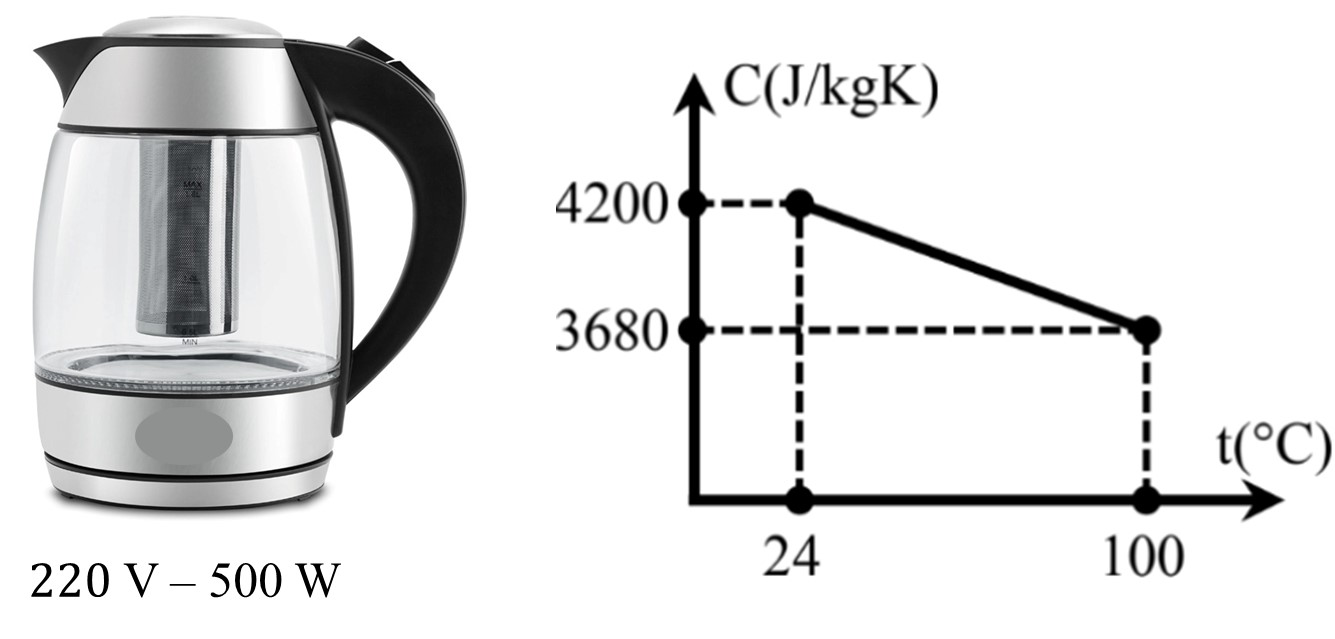
\includegraphics[scale=0.25]{../figs/FINAL-SEM1-005-15}}
Nhiệt lượng để đun sôi nước chè chiếm \SI{80}{\percent} nhiệt lượng mà dây mayso trong ấm tỏa ra. Thời gian để đun sôi nước chè là bao nhiêu phút? (lấy đến một chữ số sau dấu phẩy).
	\shortans[oly]{31,2}
	\loigiai{
		Nhiệt dung riêng trung bình là $c=\dfrac{4200+3680}{2}=\SI{3940}{\joule/\kilogram\kelvin}$.\\
		$Q=mc\Delta t=2,5\cdot3940\cdot\left(100-24\right)=\SI{748600}{\joule}$\\
		$A=\dfrac{Q}{H}=\SI{935750}{\joule}$\\
		$t=\dfrac{A}{\calP}=\dfrac{935750}{500}=\SI{1871.5}{\second}\approx\SI{31.2}{\minute}$.
	}
\end{ex}
% ===============================================================
\begin{ex}
	Một khối khí có thể tích 3 lít, được cung cấp một nhiệt lượng \SI{400}{\joule} thì nó giãn nở ở áp suất không đổi \SI{E5}{\pascal} đến thể tích \SI{4.5}{\liter}. Nội năng của khối khi này tăng thêm bao nhiêu \si{\joule}? (lấy đến chữ số hàng đơn vị).
	\shortans[oly]{250}
	\loigiai{
		$A=-p\Delta V=-10^5\cdot\left(4,5-3\right)\cdot10^{-3}=\SI{-150}{\joule}$.\\
		$\Delta U=Q+A=400-150=\SI{250}{\joule}$.
	}
\end{ex}
% ===============================================================
\begin{ex}
	\immini{Một cốc thuỷ tình hình trụ có đường kính \SI{4.0}{\centi\meter} được dùng để giác (chữa bệnh). Đốt cồn để nung nóng không khí trong cốc lên tới nhiệt độ $t_1=\SI{80}{\celsius}$ rồi úp vào lưng bệnh nhân cho kín miệng cốc. Khi không khí nguội đi thì da bị hút phồng lên. Nhiệt độ không khí trong phòng là $t=\SI{20}{\celsius}$ và áp suất khí quyển là $\SI{E5}{\pascal}$. Bỏ qua sự thay đổi thể tích khí trong cốc do da phồng lên. }
	{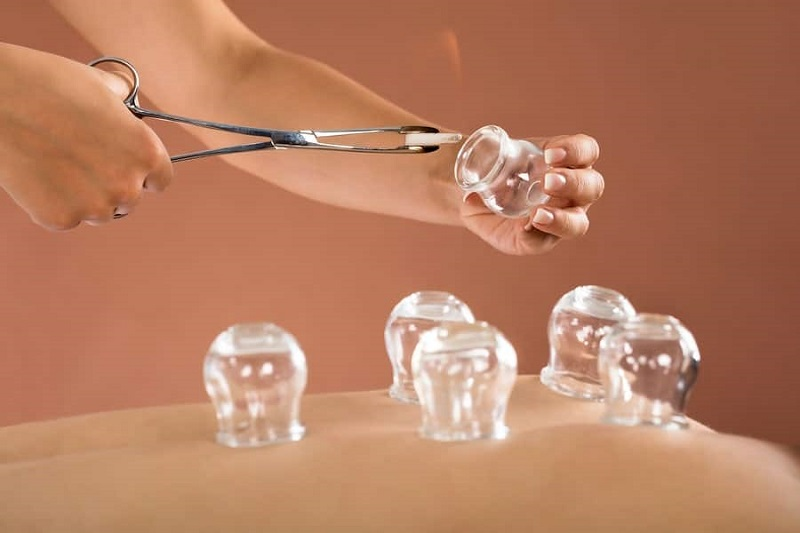
\includegraphics[scale=0.15]{../figs/FINAL-SEM1-005-16}}
	Áp lực mà cốc tác dụng lên da (do chênh lệch áp suất trong và ngoài da) là bao nhiêu \si{\newton}? (lấy đến 1 chữ số sau dấu phẩy).
	\shortans[oly]{21,4}
	\loigiai{
		\begin{center}
			\begin{tabular}{|M{5cm}|M{5cm}|M{5cm}|}
				\hline
				$p$ & $V=const$ & $T$\\
				\hline
				$\SI{E5}{\pascal}$ & & $80+273=\SI{353}{\kelvin}$\\
				\hline
				$p$ && $20+273=\SI{293}{\kelvin}$\\
				\hline
			\end{tabular}
		\end{center}
		$\dfrac{p}{T}=const\Rightarrow\dfrac{10^5}{353}=\dfrac{p}{293}\Rightarrow p\approx\SI{0.83E5}{\pascal}$\\
		$S=\pi\cdot\dfrac{d^2}{4}=\xsi{4\pi\cdot10^{-4}}{\meter^2}$\\
		$F=\left(p_0-p\right)S=\left(10^5-0,83\cdot10^5\right)\cdot4\pi\cdot10^{-4}\approx\SI{21.4}{\newton}$.
	}
\end{ex}
\Closesolutionfile{ans}
\begin{center}
	\textbf{-- HẾT --}
\end{center}
